%; whizzy paragraph -pdf xpdf -latex ./whizzypdfptex.sh
%; whizzy-paragraph "^\\\\begin{frame}\\|\\\\emtext"
% latex beamer presentation.
% platex, latex-beamer でコンパイルすることを想定。 

%     Tokyo Debian Meeting resources
%     Copyright (C) 2012 Junichi Uekawa

%     This program is free software; you can redistribute it and/or modify
%     it under the terms of the GNU General Public License as published by
%     the Free Software Foundation; either version 2 of the License, or
%     (at your option) any later version.

%     This program is distributed in the hope that it will be useful,
%     but WITHOUT ANY WARRANTY; without even the implied warreanty of
%     MERCHANTABILITY or FITNESS FOR A PARTICULAR PURPOSE.  See the
%     GNU General Public License for more details.

%     You should have received a copy of the GNU General Public License
%     along with this program; if not, write to the Free Software
%     Foundation, Inc., 51 Franklin St, Fifth Floor, Boston, MA  02110-1301 USA

\documentclass[cjk,dvipdfmx,12pt]{beamer}
\usetheme{Tokyo}
\usepackage{monthlypresentation}

%  preview (shell-command (concat "evince " (replace-regexp-in-string "tex$" "pdf"(buffer-file-name)) "&")) 
%  presentation (shell-command (concat "xpdf -fullscreen " (replace-regexp-in-string "tex$" "pdf"(buffer-file-name)) "&"))
%  presentation (shell-command (concat "evince " (replace-regexp-in-string "tex$" "pdf"(buffer-file-name)) "&"))

%http://www.naney.org/diki/dk/hyperref.html
%日本語EUC系環境の時
\AtBeginDvi{\special{pdf:tounicode EUC-UCS2}}
%シフトJIS系環境の時
%\AtBeginDvi{\special{pdf:tounicode 90ms-RKSJ-UCS2}}

\newenvironment{commandlinesmall}%
{\VerbatimEnvironment
  \begin{Sbox}\begin{minipage}{1.0\hsize}\begin{fontsize}{8}{8} \begin{BVerbatim}}%
{\end{BVerbatim}\end{fontsize}\end{minipage}\end{Sbox}
  \setlength{\fboxsep}{8pt}
% start on a new paragraph

\vspace{6pt}% skip before
\fcolorbox{dancerdarkblue}{dancerlightblue}{\TheSbox}

\vspace{6pt}% skip after
}
%end of commandlinesmall

\title{東京エリアDebian勉強会}
\subtitle{第121回 2014年12月度}
\author{野島貴英}
\date{2014年12月20日}
\logo{\includegraphics[width=8cm]{image200607/openlogo-light.eps}}

\begin{document}

\begin{frame}
\titlepage{}
\end{frame}

\begin{frame}{設営準備にご協力ください。}
会場設営よろしくおねがいします。
\end{frame}

\begin{frame}{Agenda}
 \begin{minipage}[t]{0.45\hsize}
  \begin{itemize}
   \item 注意事項
	 \begin{itemize}
	  \item 写真はセミナールーム内のみ可です。
          \item 出入りは自由でないので、もし外出したい方は、野島まで一声くださいませ。
	 \end{itemize}
   \item 事前課題発表
  \end{itemize}
 \end{minipage} 
 \begin{minipage}[t]{0.45\hsize}
  \begin{itemize}
   \item 最近あったDebian関連のイベント報告
	 \begin{itemize}
	  \item 第120回 東京エリアDebian勉強会
	 \end{itemize}
   \item Debian Trivia Quiz
   \item DebianとFedoraでパッケージをリリースするまでの話
   \item DebianからみたLinux Mint
   \item 今後のイベント
   \item 今日の宴会場所
  \end{itemize}
 \end{minipage}
\end{frame}

\section{事前課題}
\emtext{事前課題}
{\footnotesize
\begin{prework}{ henrich }
  \begin{enumerate}
  \item Q.どこで今回の勉強会の開催を知りましたか?\\
    A. 友達や知り合いから直接
  \item Q.何について聞きたい/参加者と話をしたいですか?\\
    A. \@kenhysさんの話が楽しみです! :)
  \item Q.hack timeに何をしますか?\\
    A. (回答なし)
  \end{enumerate}
\end{prework}

\begin{prework}{ 野島 }
  \begin{enumerate}
  \item Q.どこで今回の勉強会の開催を知りましたか?\\
    A. その他 (Google検索エンジンの検索結果から)
  \item Q.何について聞きたい/参加者と話をしたいですか?\\
    A. いろいろと。参加者と。
  \item Q.hack timeに何をしますか?\\
    A. RC潰しとか、翻訳とか。RCは\url{https://bugs.debian.org/release-critical/}参照。
  \end{enumerate}
\end{prework}

\begin{prework}{ knok }
  \begin{enumerate}
  \item Q.どこで今回の勉強会の開催を知りましたか?\\
    A. Debian JPのメーリングリスト
  \item Q.何について聞きたい/参加者と話をしたいですか?\\
    A. key signやります
  \item Q.hack timeに何をしますか?\\
    A. いくつかのソースの写経と、できればK\&Rスタイルの排除
  \end{enumerate}
\end{prework}

\begin{prework}{ koedoyoshida }
  \begin{enumerate}
  \item Q.どこで今回の勉強会の開催を知りましたか?\\
    A. Debian JPのメーリングリスト
  \item Q.何について聞きたい/参加者と話をしたいですか?\\
    A. パッケージング
  \item Q.hack timeに何をしますか?\\
    A. まったりメンテナンス or 翻訳
  \end{enumerate}
\end{prework}

\begin{prework}{ kenhys }
  \begin{enumerate}
  \item Q.どこで今回の勉強会の開催を知りましたか?\\
    A. Twitter (@debianjp)
  \item Q.何について聞きたい/参加者と話をしたいですか?\\
    A. ゆくゆくはDebianに一本化したいけど過渡期なためupstreamでdebian,ubuntu向けにパッケージを提供している人のdebian/管理術的なセミナーが聞きたい
  \item Q.hack timeに何をしますか?\\
    A. porterboxがらみの何か
  \end{enumerate}
\end{prework}

\begin{prework}{ wbcchsyn }
  \begin{enumerate}
  \item Q.どこで今回の勉強会の開催を知りましたか?\\
    A. 友達や知り合いから直接
  \item Q.何について聞きたい/参加者と話をしたいですか?\\
    A. 最近の状況について、情報交換
  \item Q.hack timeに何をしますか?\\
    A. Debian の開発環境構築
  \end{enumerate}
\end{prework}

\begin{prework}{ zinrai }
  \begin{enumerate}
  \item Q.どこで今回の勉強会の開催を知りましたか?\\
    A. その他
  \item Q.何について聞きたい/参加者と話をしたいですか?\\
    A. systemd
  \item Q.hack timeに何をしますか?\\
    A. drone+dockerでCIを試してみる
  \end{enumerate}
\end{prework}

\begin{prework}{ alohaug }
  \begin{enumerate}
  \item Q.どこで今回の勉強会の開催を知りましたか?\\
    A. その他
  \item Q.何について聞きたい/参加者と話をしたいですか?\\
    A. Gnukの現状の紹介がしたいです。
  \item Q.hack timeに何をしますか?\\
    A. Gnukのツール作りでハマっていることを相談したいです。
  \end{enumerate}
\end{prework}

\begin{prework}{ munepi }
  \begin{enumerate}
  \item Q.どこで今回の勉強会の開催を知りましたか?\\
    A. Debian JPのメーリングリスト
  \item Q.何について聞きたい/参加者と話をしたいですか?\\
    A. DebianとFedoraパッケージングのお話
  \item Q.hack timeに何をしますか?\\
    A. 勉強会資料用\LaTeX スタイルの改善、クラスファイルの作成(案)
  \end{enumerate}
\end{prework}

\begin{prework}{yy\_y\_ja\_jp }
  \begin{enumerate}
  \item Q.どこで今回の勉強会の開催を知りましたか?\\
    A. その他
  \item Q.何について聞きたい/参加者と話をしたいですか?\\
    A. Debian
  \item Q.hack timeに何をしますか?\\
    A. DDTSS(\url{http://ddtp.debian.net/ddtss/index.cgi/ja})
  \end{enumerate}
\end{prework}

}

\section{イベント報告}
\emtext{イベント報告}

\begin{frame}{第120回東京エリアDebian勉強会}

\begin{itemize}
\item 場所はスクウェア・エニックスさんのセミナルームをお借りしての開催でした。
\item 参加者は10名でした。
\item セミナ内容は野島により、DebianとArch Linuxの比較を行ったことについて語りました。
\item 残りの時間でhack timeを行い、成果発表をしました。
\item 宴会の代わりに、「やよい軒 新宿明治通り店」で夕食会をやりました。
\end{itemize} 
  
\end{frame}

\begin{frame}{第120回東京エリアDebian勉強会(つづき)}

 Arch LinuxがOSC Tokyoの若い参加に何故人気があるのか、Debianとどう違い、どういうニーズがあるのか?について考察できたように思います。他のディストリビューションと比較すると、Debianの立ち位置、取り込んだ方が良い機能などがわかって良いかと思います。
  
\end{frame}


\section{Debian Trivia Quiz}
\emtext{Debian Trivia Quiz}
\begin{frame}{Debian Trivia Quiz}

  Debian の常識、もちろん知ってますよね?
知らないなんて恥ずかしくて、知らないとは言えないあんなことやこんなこと、
みんなで確認してみましょう。

今回の出題範囲は\url{debian-devel-announce@lists.debian.org},
\url{debian-news@lists.debian.org} に投稿された
内容などからです。

\end{frame}

\subsection{問題}

%; whizzy-master ../debianmeetingresume201211.tex
% $B0J>e$N@_Dj$r$7$F$$$k$?$a!"$3$N%U%!%$%k$G(B M-x whizzytex $B$9$k$H!"(Bwhizzytex$B$,MxMQ$G$-$^$9!#(B
%

\santaku
{DebConf13 $B$N3+:ECO$H3+:EF|$O!)(B}
{$BF|K\!"El5~ET(B 6$B7n(B20$BF|(B}
{$B%K%+%i%0%"(B $B%^%J%0%"(B 7$B7n(B8-14$BF|(B}
{$B%9%$%9!"%t%)!<%^%k%-%e(B 8$B7n(B11-18$BF|(B}
{C}
{$B%K%+%i%0%"$O(BDebConf12$B$N3+:ECO$G$9!#(B
DebConf13$B$O%9%$%9$N%-%c%s%WCO$G3+:E$G$9!#(B
6/20$B$O3'$5$sM=Dj$r6u$1$F$*$-$^$7$g$&!#(B}

\santaku
{$B@$3&$N(BWeb$B%5!<%P$G:G$b?M5$$N$"$k(BLinux $B%G%#%9%H%j%S%e!<%7%g%s(B(W3Techs$BD4$Y(B)$B$O!)(B}
{CentOS}
{Debian}
{Ubuntu}
{B}
{\url{http://w3techs.com/technologies/history_details/os-linux}$B$K7k2L$N%0%i%U$,$"$j$^$9!#(B
$B8=:_(B Linux $B$r;HMQ$7$F$$$k(B web $B%5!<%P$N(B 32.9\% $B$,(B Debian $B$rMxMQ$7$F$*$j!"$=$N3d9g$O8=:_$bA}2C$rB3$1$F$$$k$=$&$G$9!#(B}

\santaku
{Ben Hutchings $B$5$s$,<!4|(B Debian $B0BDjHG$H0l=o$K=P2Y$5$l$k(B Linux $B%+!<%M%k$K(B (3.2 $B7ONs$N(B mainline $B$K$OL5$$(B) $BDI2C5!G=$,Ek:\$5$l$kM=Dj$G$"$k$H=R$Y$F$$$^$9!#(B
$BB?$/$NDI2CE@$NCf$K4^$^$l$J$$$b$N$O2?!)(B}
{PREEMPT\_RT}
{Hyper-V guest drivers$B$N6/2=(B}
{ARM64/AArch64$B%"!<%-%F%/%A%c%5%]!<%H(B}
{C}
{Ben Hutchings $B$5$s$O(BDebian $B%+!<%M%k%A!<%`$N%a%s%P!<$G$"$j!"(Bkernel.org $B$N(B 3.2.y $B0BDjHG7ONs$N%a%s%F%J$G$9!#(BHyper-V guest drivers$B$O(Bmainline kernel$B$G(B3.2$B$K$b4^$^$l$F$$$^$9$,!"$h$j2~A1$5$l$?(B3.4$B$+$i$N=$@5$,F3F~$5$l$^$9!#(B
PREEMPT\_RT$B$O%O!<%I%j%"%k%?%$%`$r<B8=$9$k$?$a$N(BPatch$B!"(B
linux-image-rt-amd64 , linux-image-rt-686-pae $B$N(Bmetapackage$B$G;HMQ$G$-$^$9!#(B
$B?7$7$$(BARM 64$B%S%C%H%"!<%-%F%/%A%c%5%]!<%H$O(Bmainline kernel 3.7$B$+$i(B}

\santaku
{Wookey$B$5$s$,%"%J%&%s%9$7$?(Balpha$BHG$N(BDebian port arm64 image$B$O!)(B}
{Debian/Ubuntu port image}
{Debian/KFreeBSD port image}
{Debian/GnuHurd port image}
{A}
{self-bootstrapp(non x86)$BBP1~$H$N$3$H$G$9!#(B\url{http://wiki.debian.org/Arm64Port}$B$G%9%F!<%?%9$,3NG'$G$-$^$9!#(B}

\santaku
{700,000$BHVL\$N%P%0$,Js9p$5$l$?F|$rEv$F$k(B700000thBugContest$B$N7k2L$,=P$^$7$?!#$=$NM=A[F|$HJs9pF|$O!)(B}
{$BM=A[F|(B:2013/02/04$B!"Js9pF|(B:2013/02/14}
{$BM=A[F|(B:2013/02/07$B!"Js9pF|(B:2013/02/14}
{$BM=A[F|(B:2013/02/14$B!"Js9pF|(B:2013/02/07}
{C}
{$B:G$b6a$$(B2013/02/14$B$rM=A[$7$?(BChristian Perrier$B$5$s$,Ev$F$^$7$?!#7k2L$O(B\url{http://wiki.debian.org/700000thBugContest}$B$G8x3+$5$l$F$$$^$9!#(B
$B$^$?!"(B800,000/1,000,000$BHVL\$N%P%0$,Js9p$5$l$kF|$rEv$F$k%3%s%F%9%H(B\url{http://wiki.debian.org/800000thBugContest}$B$b3+:E$5$l$F$$$^$9!#(B}

\santaku
{master.debian.org$B$,?7$7$$5!3#$K0\9T$5$l$^$7$?!#$3$l$O2?$N%5!<%P$G$7$g$&$+(B $B!)(B}
{@debian.org$B$N%a!<%k%5!<%P(B}
{$B%Q%C%1!<%8$N%^%9%?!<%5!<%P(B}
{$B%Q%C%1!<%8$N%9%]%s%5!<(B(mentor)$B$rC5$9%5!<%P(B}
{A}
{$B8E$$%5!<%P$O%G%#%9%/>c32Ey$,$"$C$?$N$G!"<wL?$HH=CG$5$l!"%G!<%?$,B;<:$9$kA0$K?7$7$$%5!<%P$K0\9T$5$l$^$7$?!#(Bftp-master.debian.org$B$O(BDebian$B$N(B official package $B%j%]%8%H%j$G$9!#%Q%C%1!<%8$N%9%]%s%5!<(B(mentor)$B$rC5$9$N$O(Bmentors.debian.net$B!#(B }

\santaku
{pbuilder$B$K(Bclang support$B$,DI2C$5$l$^$7$?!#C/$,=q$$$?%Q%C%A$G$7$g$&$+!)(B}
{Sylvestre Ledru}
{Junichi Uekawa}
{Hideki Yamane}
{C}
{Debian$B$N(BClang$B%5%]!<%H$OCe!9$H?J$s$G$$$^$9!#(B}

\santaku
{DPN - 2013$BG/(B3$B7n(B4$BF|9f$K<h$j>e$2$i$l$?F|K\$N%$%Y%s%H$O(B}
{Open Source Conference 2013 Tokyo/Spring}
{Open Source Conference 2013 Hamamatu}
{Open Source Conference 2013 Tokushima}
{A}
{\url{http://henrich-on-debian.blogspot.jp/2013/02/open-source-conference-2013-tokyospring.html} $B>\:Y$O8e$[$I!#(B}



\section{DebianとFedoraでパッケージをリリースするまでの話}
\emtext{DebianとFedoraでパッケージをリリースするまでの話}

\section{DebianからみたLinux Mint}
\emtext{DebianからみたLinux Mint}

\begin{frame}{Linux Mint!?}

  OSC Tokyoにて、ブースに来た若い方々に「どんなディストリビューション使ってる?」って聞いた時の結果:

\begin{itemize}
 \item Arch Linux (←結構多い)
 \item Linux MINT (←次に多い)
\end{itemize}

\begin{center}
{\LARGE (前回に引き続き)Debianじゃない!!ナゼ!? ナンデ!?}
\end{center}
\end{frame}

\begin{frame}{というわけでLinux Mint}

 Debianに、Linux Mintの良いところを取り入れるべく、比較しながら調べてみました。
  
\end{frame}

\begin{frame}{Linux Mintとは}

  Linux Mintは、
\begin{itemize}
\item i686/x86\_64で使えるLinuxディストリビューションの1つであり、
\item debian/ubuntuをうまく活用して作られている
\end{itemize}
ディストリビューションです。
\end{frame}

\begin{frame}{とりあえず使ってみる}

  DebianのKVM環境を使って動かすやり方を第121回東京エリアDebian勉強会資料
  (\url{http://tokyodebian.alioth.debian.org/pdf/ debianmeetingresume201412.pdf})
に載せてますので、参照くださいませ。
    
\end{frame}

\begin{frame}{動いた!}

\begin{figure}[H]
\centering
 \includegraphics[width=0.7\hsize]{image201412/mint-setupcomplete.png}
\caption{Linux Mint 17.1 のMATE版が動作}
\end{figure}
\end{frame}

\begin{frame}{動かなかった!}

  Linux Mint 17.1のcinnamon版はdebian sidのKVMの元では、cirrus/qxl共に動作が不安定で使えなかったです...orz。
  \begin{center}
   {\LARGE 将来に期待!}
  \end{center}
  
\end{frame}

\begin{frame}{ちょっとだけハマりポイント}

\begin{itemize}
\item virt-viewerで画面描画がおかしい場合は、cirrusの代わりにqxlをvirt側のxml設定ファイルに記述すると非常に良くなる事があります。
\item 音が無くて寂しい場合は、ac97を指定して、vncプロトコルの代わりにspiceプロトコルを指定すると、virt-viewerから音が出ます。
\item ディスクは最低でも9GBytes以上、メモリは1GBytes以上割り当てないとインストールに失敗します。(マニュアルに明記が無いのでハマります)
\end{itemize}
  
\end{frame}

\begin{frame}[containsverbatim]{ちょっとだけハマりポイント}

 仮想側のsoundデバイスを指定し、qxlをビデオドライバに指定して、spiceプロトコルを有効にする設定の例:
  
\begin{commandlinesmall}
$ sudo virt edit mint-01
...xmlファイル中...
 <graphics type='spice' port='5900' autoport='no'>
   <mouse mode='server'/>
   <clipboard copypaste='yes'/>
 </graphics>
 <sound model='ac97'>
 </sound>
 <video>
   <model type='qxl' ram='65536' vram='65536' heads='1'>
     <acceleration accel3d='yes' accel2d='yes'/>
   </model>
 </video>
...xmlファイル中...
\end{commandlinesmall}

\end{frame}


\begin{frame}{参考:コード名}

  Linux Mint はコード名に頭文字がA-Zの順番で決まる女性の名前を使うんだそうです。
 前回のバージョンLinux Mint 17はOiana。今回の最新バージョン17.1はRebbeca。\\
  参考:Debianはトイ・ストーリーのキャラクタ名。

\end{frame}

\begin{frame}{参考:日本語IMは?}

 今までLinux Mintの日本語IM導入はLinux Mint Japanチームの追加パッケージを別途導入しなければなりませんでしたが、Linux Mint 17.1からはログイン後のメニューから、「設定」→「Languages」で起動するユーティリティでメニューから簡単設定出来るようになった模様です。
  
\end{frame}

\begin{frame}{参考:日本語IMは?}

 \begin{figure}[H]
\centering
 \includegraphics[width=0.7\hsize]{image201412/mint-im-setup.png}
\caption{Linux Mint 17.1 の日本語IM設定/導入メニュー}
\end{figure}
  
\end{frame}

\begin{frame}{Linux MintとUbuntu/Debianの関係}

\begin{figure}[H]
\centering
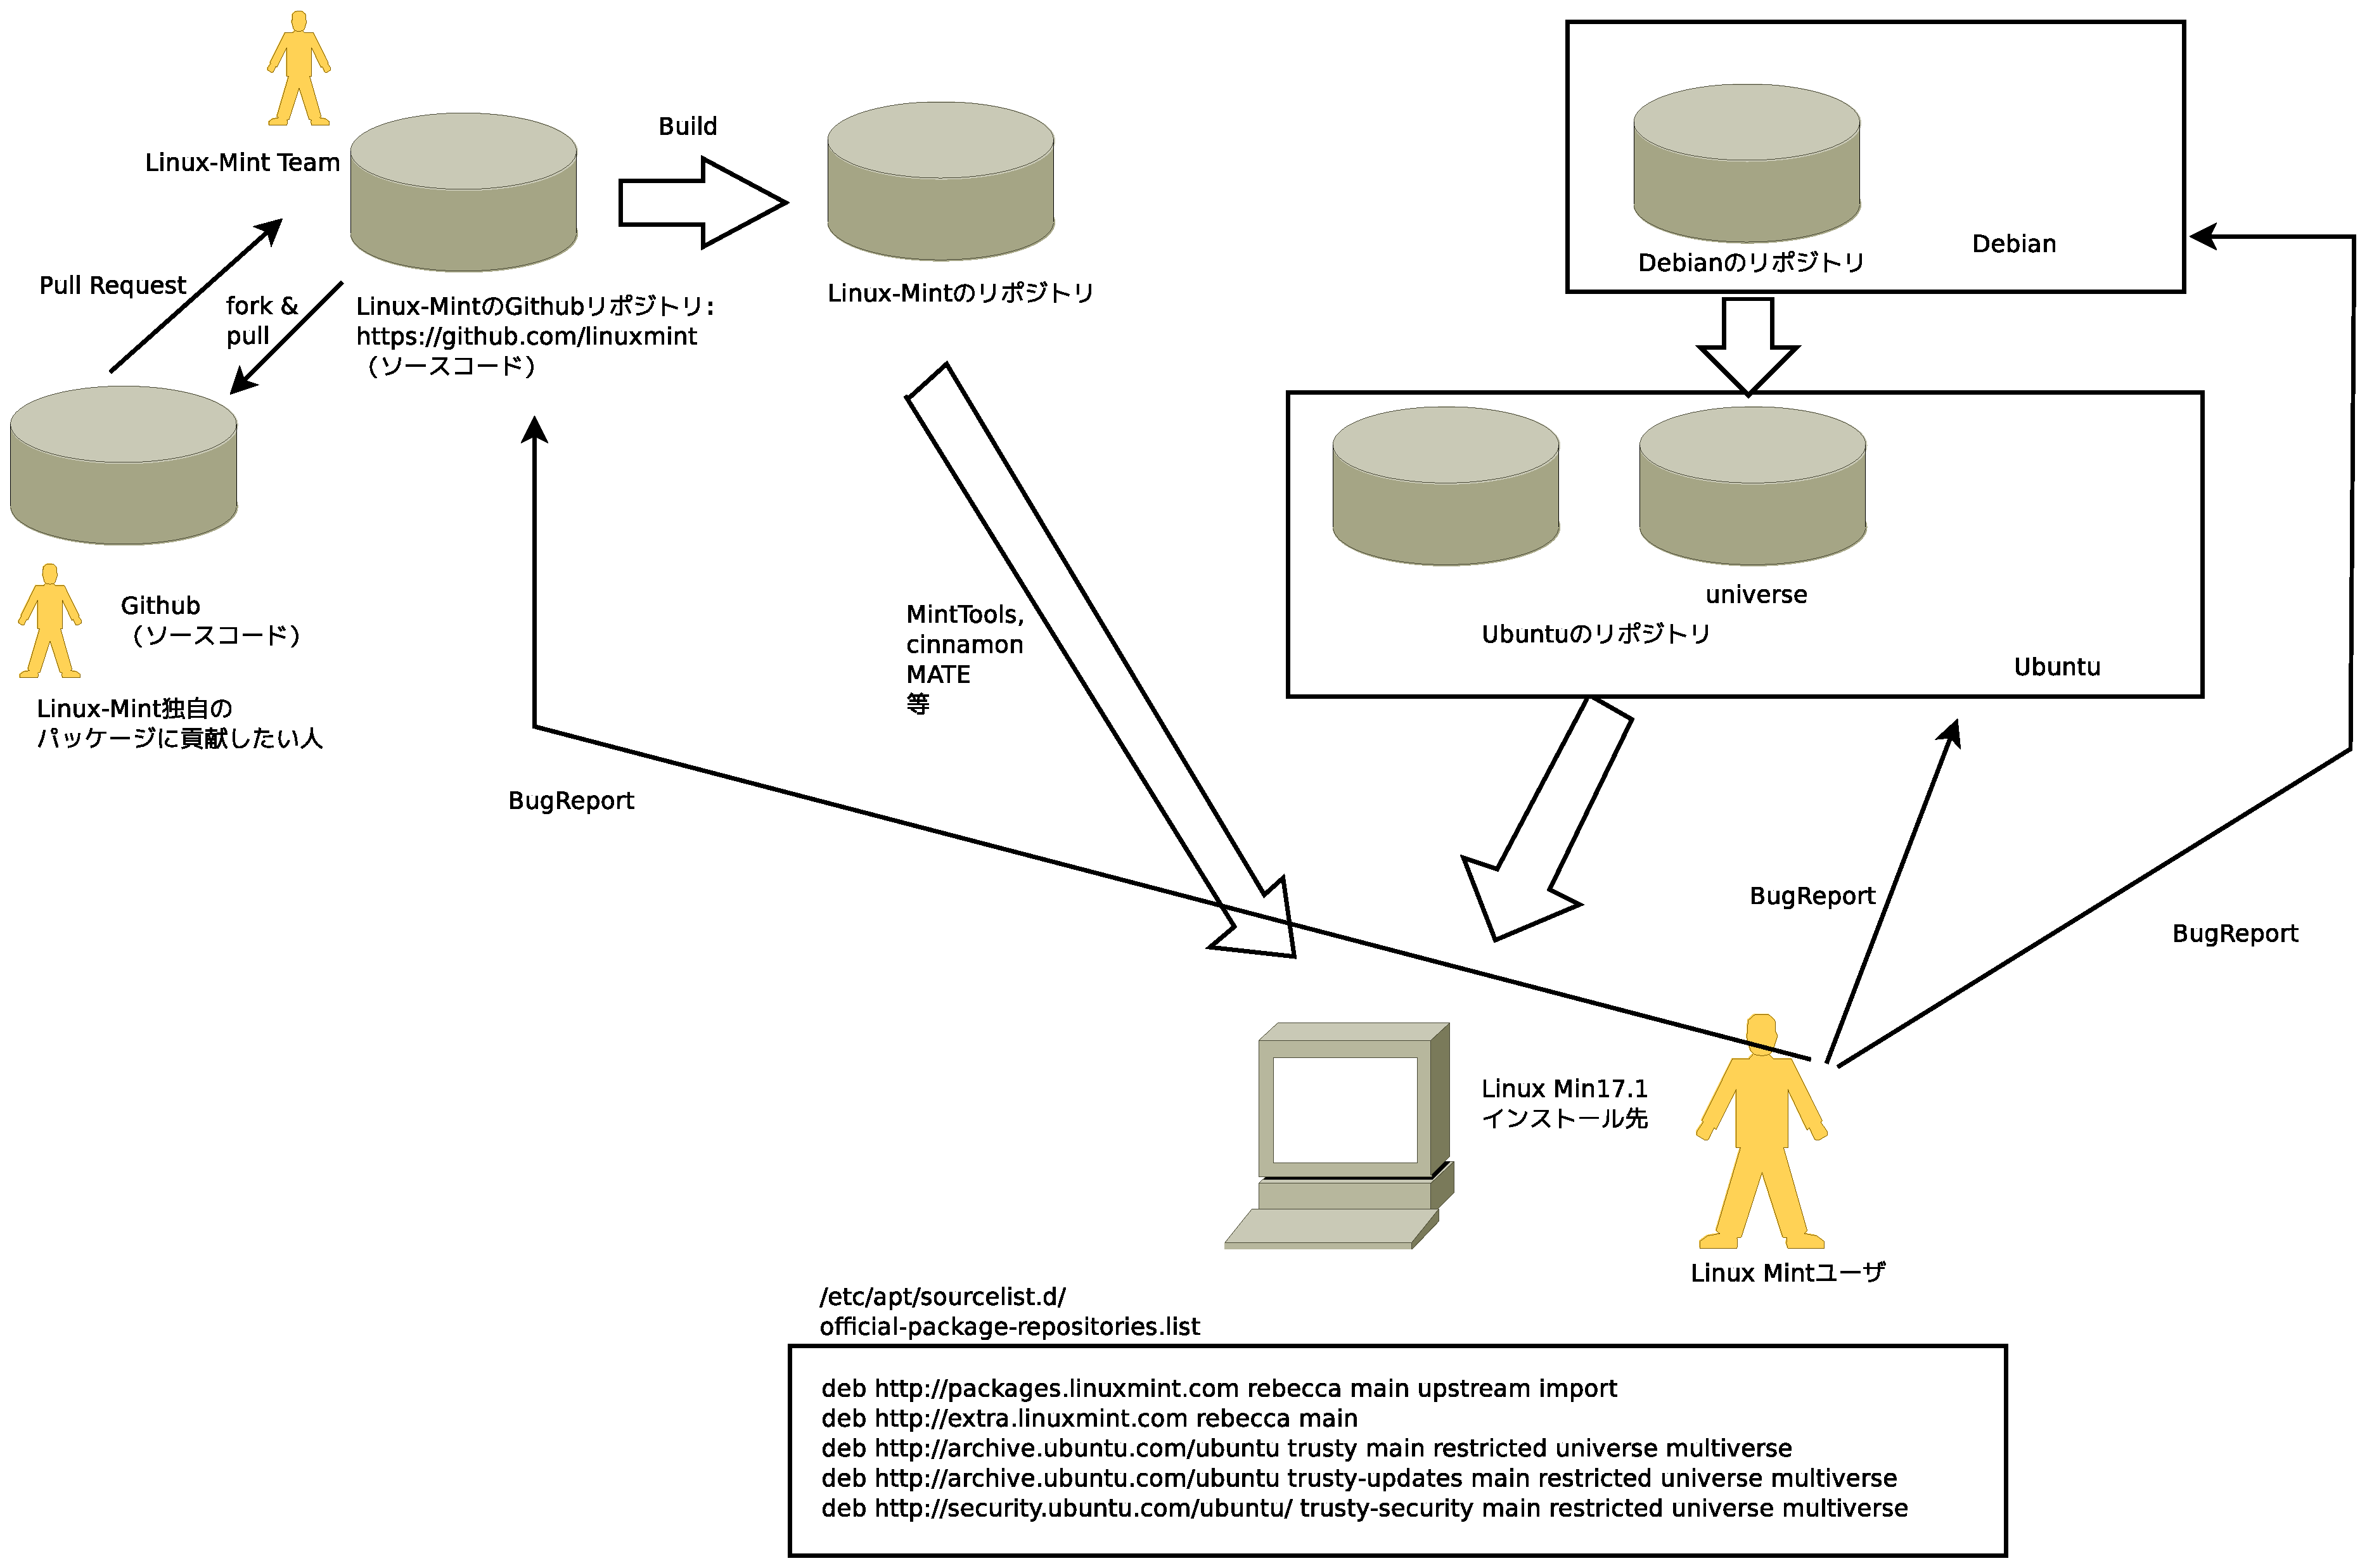
\includegraphics[width=0.7\hsize]{image201412/mint-construct.eps}
\caption{Linux MintとUbuntu/Debianの関係}
\end{figure}
  
\end{frame}

\begin{frame}{使ってわかるLinux Mintの良さ}

\begin{itemize}
\item Linux Mint側でメンテナンスされている部分の作りが非常に丁寧。GUIとシステム連携の完成度が高い。
 \item Linux Mint側のcommunityサイトは、投票システムを搭載しており、ユーザの投稿のランキングなどの様々な統計がすぐわかる。アイデア投稿もあり、アイデアはすぐに他ユーザの手により評価される。
\end{itemize}
\end{frame}

\begin{frame}{Debianにcinnamon}

  Debianにcinnamon入れたらひょっとしてLinux Mintになる?\\
  wktk...
 
\end{frame}  

\begin{frame}[containsverbatim]{Debianにcinnamon}

\begin{description}
\item [Step 1.] Debian sidをデスクトップ環境を全く導入しない最小限の構成で導入。
\item [Step 2.] cinnamonデスクトップ環境を導入。
  \begin{commandlinesmall}
$ sudo aptitude install cinnamon-desktop-envirionment
  \end{commandlinesmall}
\end{description}

\begin{center}
\LARGE とっても簡単!
\end{center}
\end{frame}  

\begin{frame}{Debianにcinnamon}

できた!

\begin{figure}[H]
\centering
\includegraphics[width=0.6\hsize]{image201412/debian-cinnamon.png}  
\caption{Debianにcinnamonを導入}\label{fig:debian-cinnamon}
\end{figure} 
  
\end{frame}  

\begin{frame}{Debianにcinnamon感想}

  \begin{itemize}
  \item やっぱりDebianのルックアンドフィール。
  \item 考え方もDebianの他のデスクトップ環境と同じポリシー。
  \item OS側との連携度合いも、Debian流。
  \end{itemize}
  
\end{frame}  

\begin{frame}{Debianにcinnamon感想}

  \centering
  うーん、Linux MintをDebianに引き込むにはcinnamonだけじゃダメか...
  
\end{frame}  

\begin{frame}{まとめ}

 Linux Mintの良いところである、
  
\begin{itemize}  
\item Linux Mint communityのサイト(WEB上の投票システムとか、アイデア出しとか)
\item Linux Mint並にGUIとシステム管理が丁寧に統合されたデスクトップ環境の構成
\end{itemize}

はDebianを考えるときに参考になりました!

\end{frame}  

\section{今後のイベント}
\emtext{今後のイベント}
\begin{frame}{今後のイベント}
\begin{itemize}
 \item 関西エリアDebian勉強会
 \item 東京エリアDebian勉強会 
\end{itemize}
\end{frame}

\section{今日の宴会場所}
\emtext{今日の宴会場所}
\begin{frame}{今日の宴会場所}
未定
\end{frame}

\end{document}

;;; Local Variables: ***
;;; outline-regexp: "\\([ 	]*\\\\\\(documentstyle\\|documentclass\\|emtext\\|section\\|begin{frame}\\)\\*?[ 	]*[[{]\\|[]+\\)" ***
;;; End: ***
